%% 
%%	This is file 'beamer_sample.tex'
%%	according to an MPIDR's PowerPoint template (?)
%%	
%%	by Eric Naujoks
%%
%%	Problems, bugs and comments to 
%%	naujoks@demogr.mpg.de
%%

%%%%%%%%%%%%%%%%%%%%%%%%%%%%%%%%%%
%%	Praelegomena								%%
%%%%%%%%%%%%%%%%%%%%%%%%%%%%%%%%%%
%%	- Make sure that you use utf8-encoding for all your .tex-files!!! (TeXnicCenter since version 2.0)
%%	- TeXnicCenter update: MPIDR intranet > Hard- & Sortfware > Software > Script and text editors > TeXnicCenter

\documentclass[20pt]{beamer}

\usepackage[ngerman,english]{babel}
\usepackage{graphicx}
\usepackage{tikz}
\usepackage{animate} 
\usepackage[normalem]{ulem}
\geometry{paperwidth=10in, paperheight=7.5in}
\usepackage{hyperref}
\usepackage[utf8]{inputenc}
\usepackage{movie15}
%\usepackage{multimedia}
\usepackage[mpidr]{./mpidr/beamerthemeMPIDR}


%% Declaring title and author
\title{A model of lifetimes}
\subtitle{Tim Riffe\\ Lab of Population Health}		%% subtitle means author in
% this file...
% :/


%%	the institute's logo
\renewcommand{\mylogo}{
\includegraphics[width=4.7in]{mpidr_logo_colour_en}}


%%	should be the very last package to be loaded
\usepackage{hyperref}

%%%%%%%%%%%%%%%%%%%%%%%%%%%%%%%%%%
%%	Beginning of the document		%%
%%%%%%%%%%%%%%%%%%%%%%%%%%%%%%%%%%
\begin{document}

%%	titlepage - fixed frame:
%%	========================
\begin{frame}
	\titlepage
\end{frame}

%%	TOC:
%%	====
\begin{frame}%{Table of Contents}
  \begin{description}
    \item<1->{\textbf{APC}:} well-known. Aligned to time of birth.
    \item<2->{\textbf{TPD}:} like APC, but aligned to death.
    \item<3->{\textbf{ATL}:} shows variation over the lifespan, but not in
    calendar time.
    \item<4->{\textbf{APCTDL}:} everything in one redundant 3d relationship.
    \item<5->{\textbf{demonstration:}} a bottled example.
  \end{description}
\end{frame}

%%	section 1:
%%	APC
\section{APC}
% typical APC setup
\begin{frame}
\frametitle{APC, an old friend}
\begin{figure}[b]
    \centering
       % figure made in R/APClab.R
    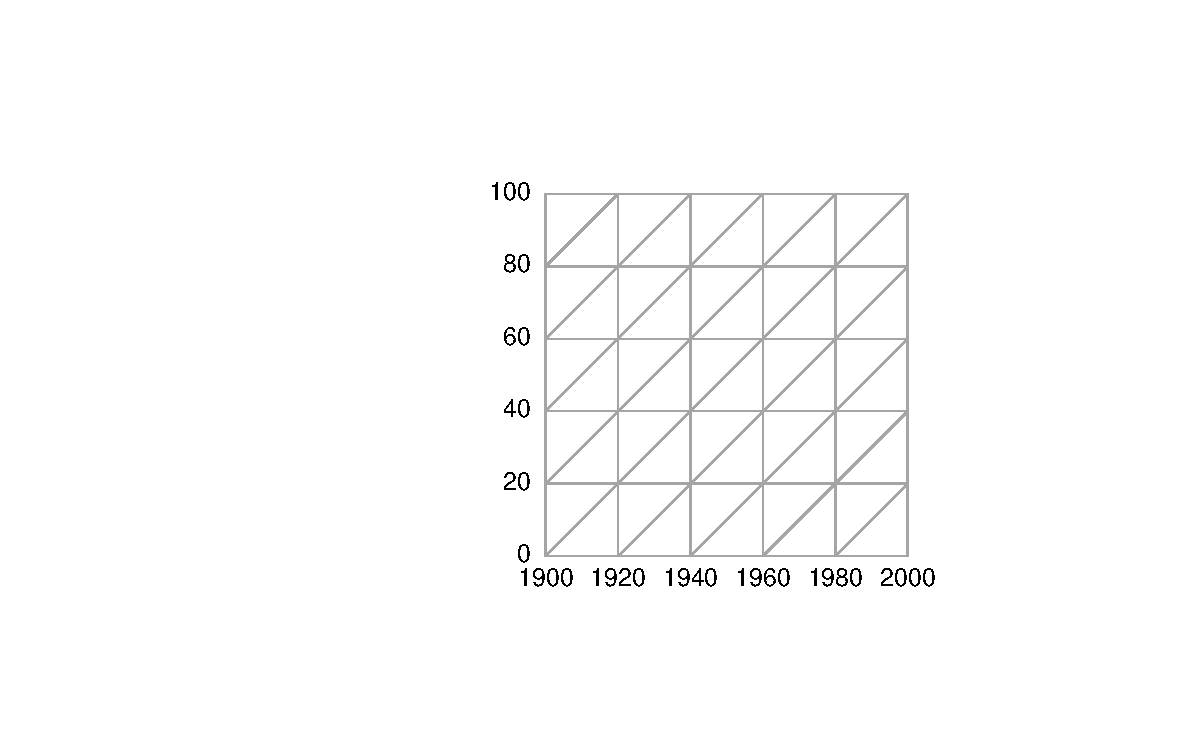
\includegraphics{Figures/LabPres/APC1.pdf}
    %\caption{An APC diagram}
\end{figure} 
\end{frame}

% observed, with lifelines
\begin{frame}
\frametitle{APC, an old friend}
\begin{figure}[b]
    \centering
      % figure made in R/APClab.R
    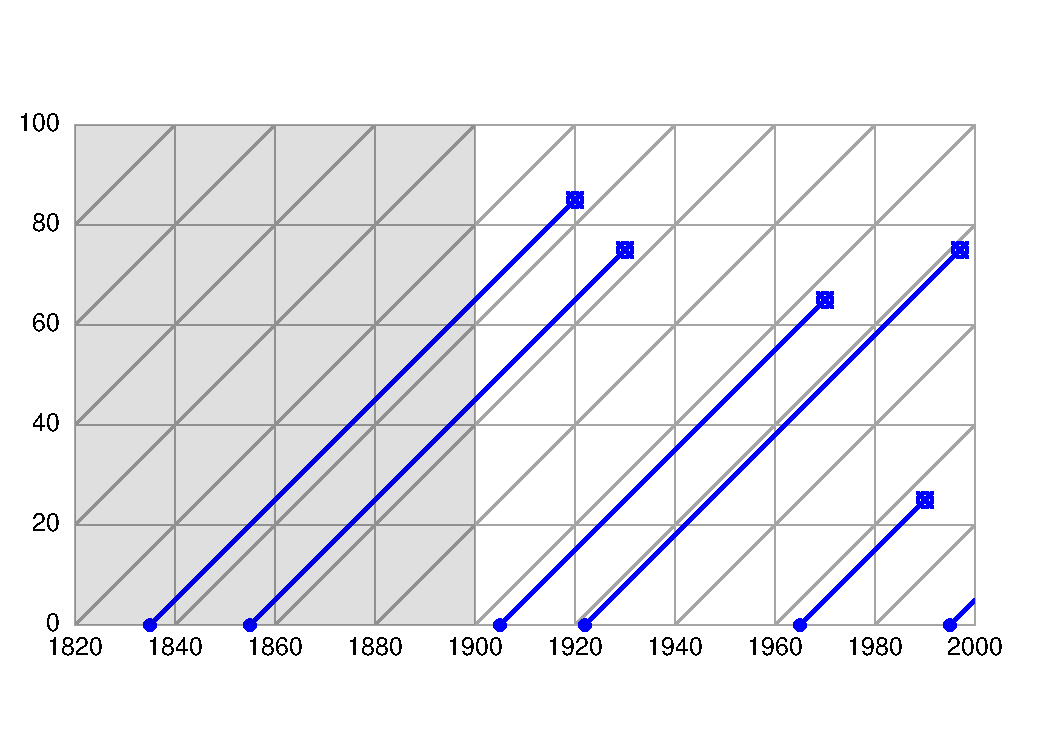
\includegraphics{Figures/LabPres/APC2.pdf}
    %\caption{Lifelines in the APC diagram}
\end{figure} 
\end{frame}

% past, observed,
\begin{frame}
\frametitle{APC, an old friend}
\begin{figure}[b]
    \centering
       % figure made in R/APClab.R
    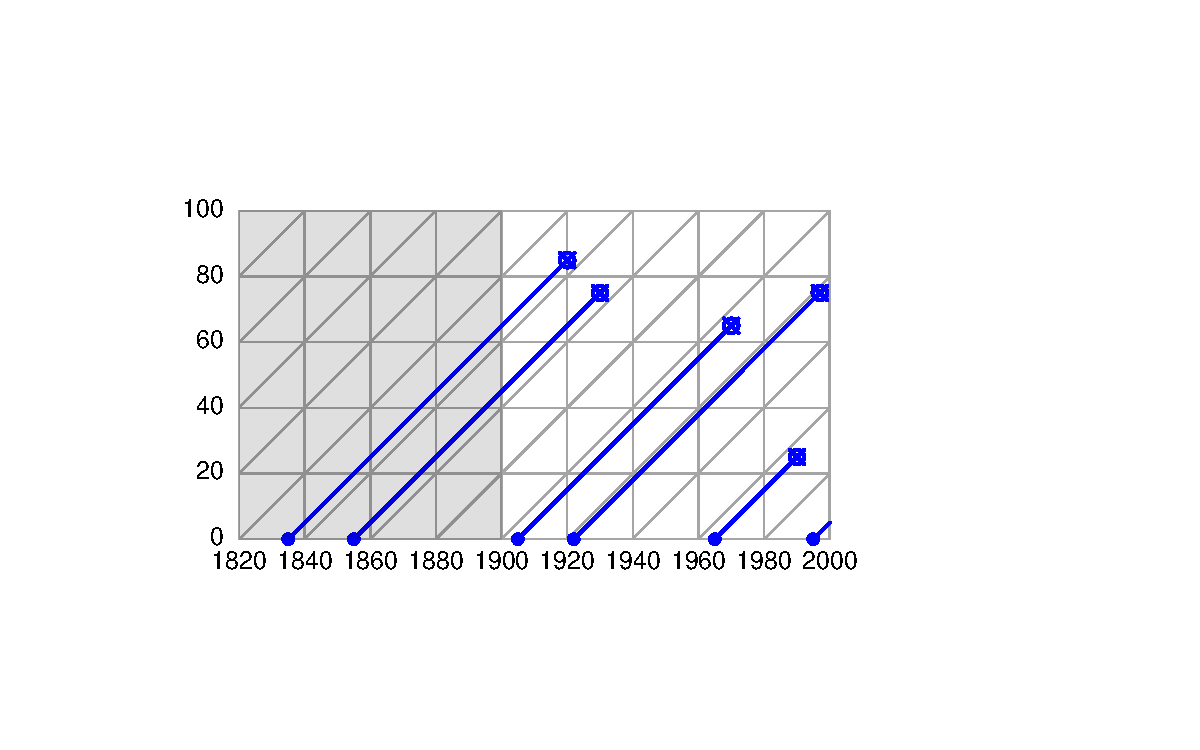
\includegraphics{Figures/LabPres/APC3.pdf}
   %\caption{Lifelines in the APC diagram, past}
\end{figure} 
\end{frame}

% past, observed, future
\begin{frame}
\frametitle{APC, an old friend}
\begin{figure}[b]
    \centering
       % figure made in R/APClab.R
    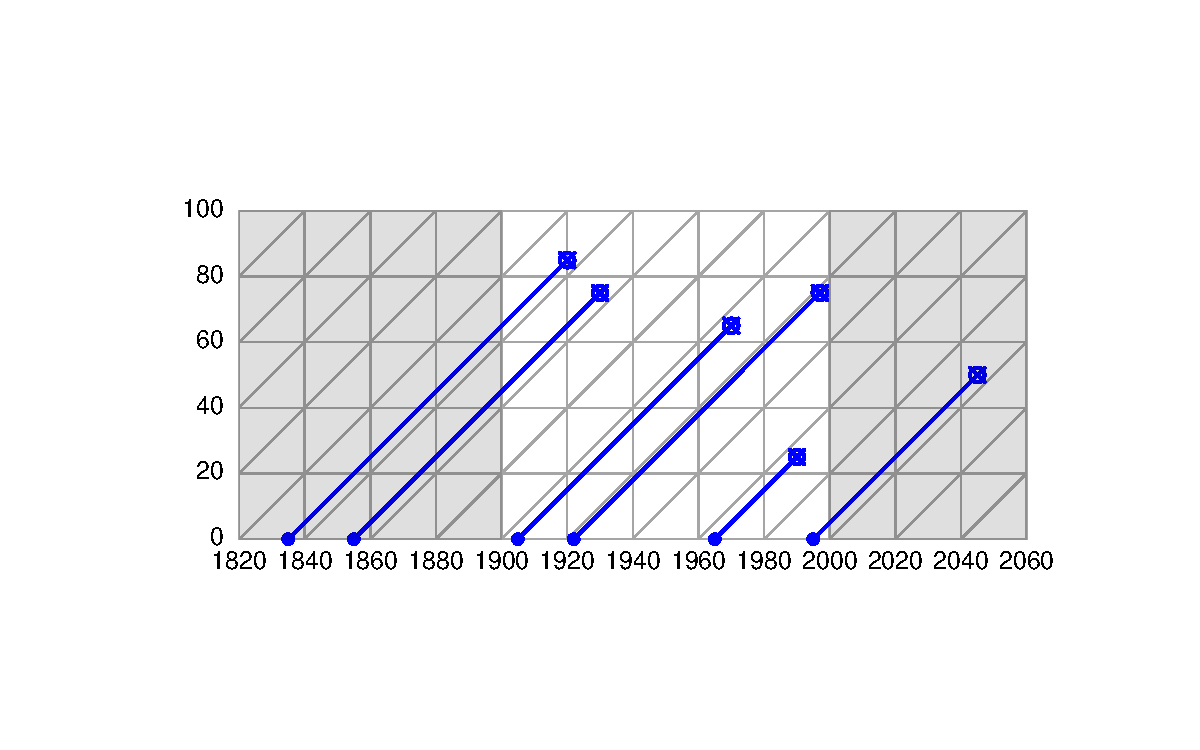
\includegraphics{Figures/LabPres/APC4.pdf}
   % \caption{Lifelines in the APC diagram, past and future}
\end{figure} 
\end{frame}

% Equilateral Lexis (Zeuner, Perozzo, Ryder)
\begin{frame}
\frametitle{APC, an old friend}
\begin{figure}[b]
    \centering
    % figure made in R/APClab.R
    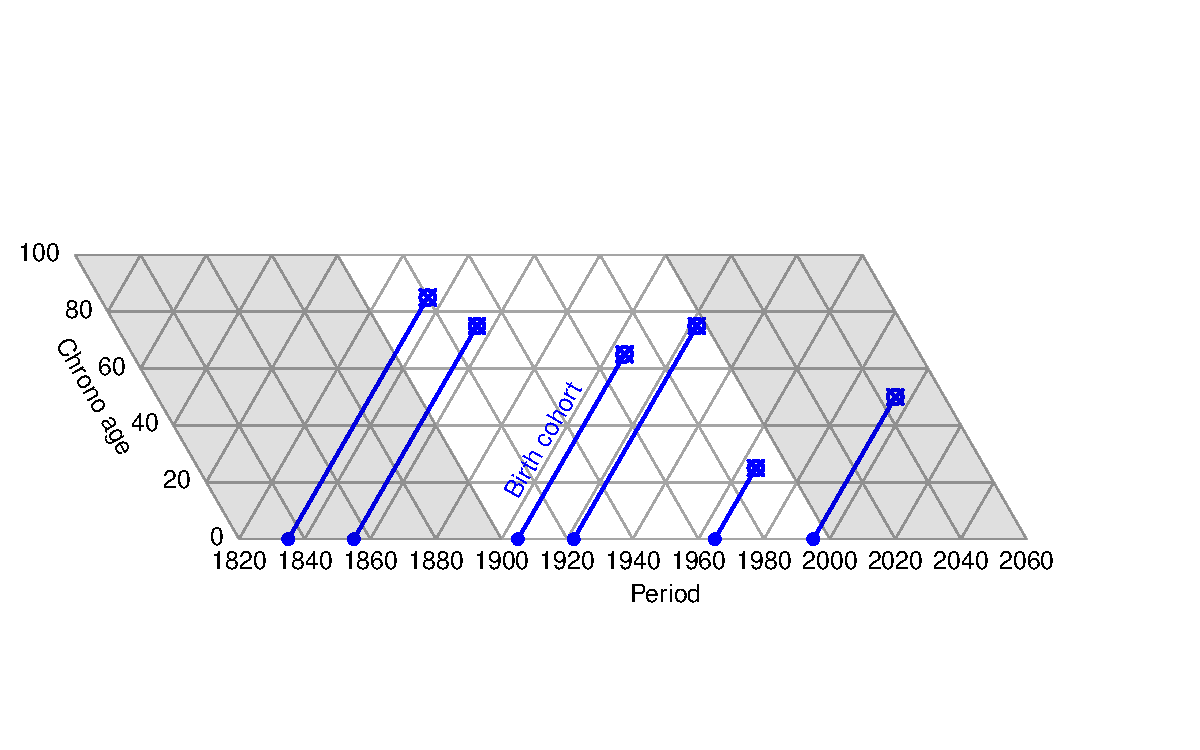
\includegraphics{Figures/LabPres/APC5.pdf}
    %\caption{Lifelines in the equilateral APC diagram}
\end{figure} 
\end{frame}

\begin{frame}
\frametitle{APC, the greatest and best}
\begin{figure}[b]
    \centering
     % figure modified from a 600dpi scan of the original, HT interlibrary loan,
     % and Stanford university library.
    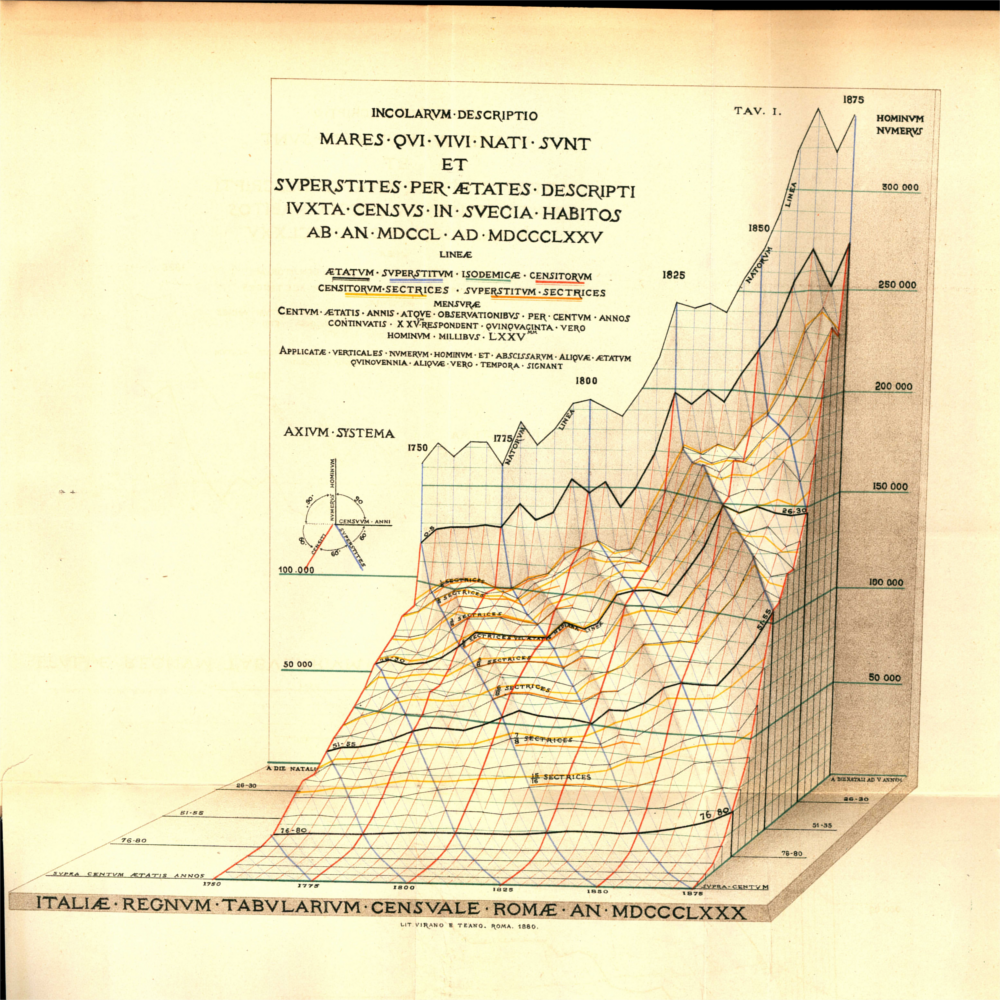
\includegraphics[scale=.5]{Figures/LabPres/Perozzo1000px_cropped_adj.png}
\end{figure} 
\end{frame}

%%	TPD
\section{TPD}
%\begin{frame}
%\frametitle{The inverse relationship}
%\begin{figure}[b]
%    \centering
    % figure made in R/LexisStandard.R
%    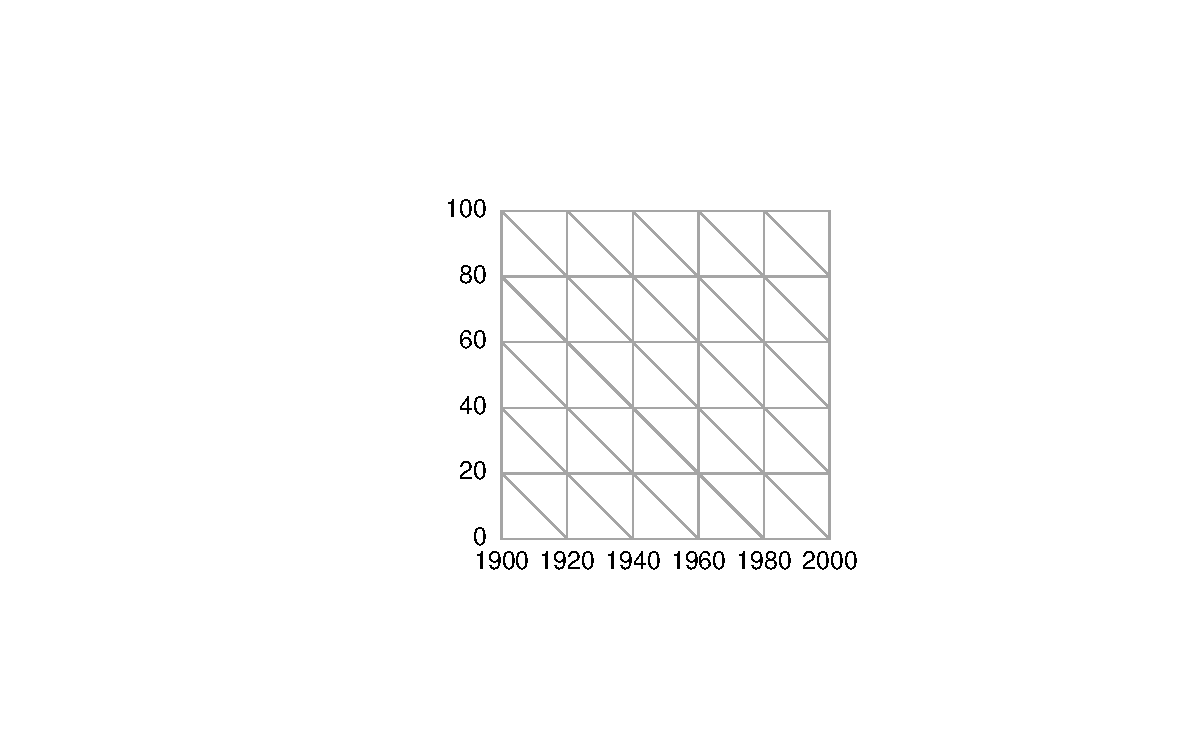
\includegraphics[scale=.9]{Figures/LabPres/TPD1.pdf}
%    \caption{A TPD diagram}
%\end{figure} 
%\end{frame}

%\begin{frame}
%\begin{figure}[hpt!]
%\includemovie[autoplay]{5in}{4in}{Figures/LabPres/Timelapsehourglass.mp4}                                   
%\end{figure}
%\end{frame}
%
\begin{frame} 
\frametitle{realign lifelines}
\begin{figure}
    \centering
  \animategraphics[height=5in]{36}{Figures/LabPres/AnimateLifeLines/frame_}{1}{95}
\end{figure} 
\end{frame} 

\begin{frame}
\frametitle{TPD, the inverse relationship}
\begin{figure}[b]
    \centering
    % figure made in R/TPDlab.R
    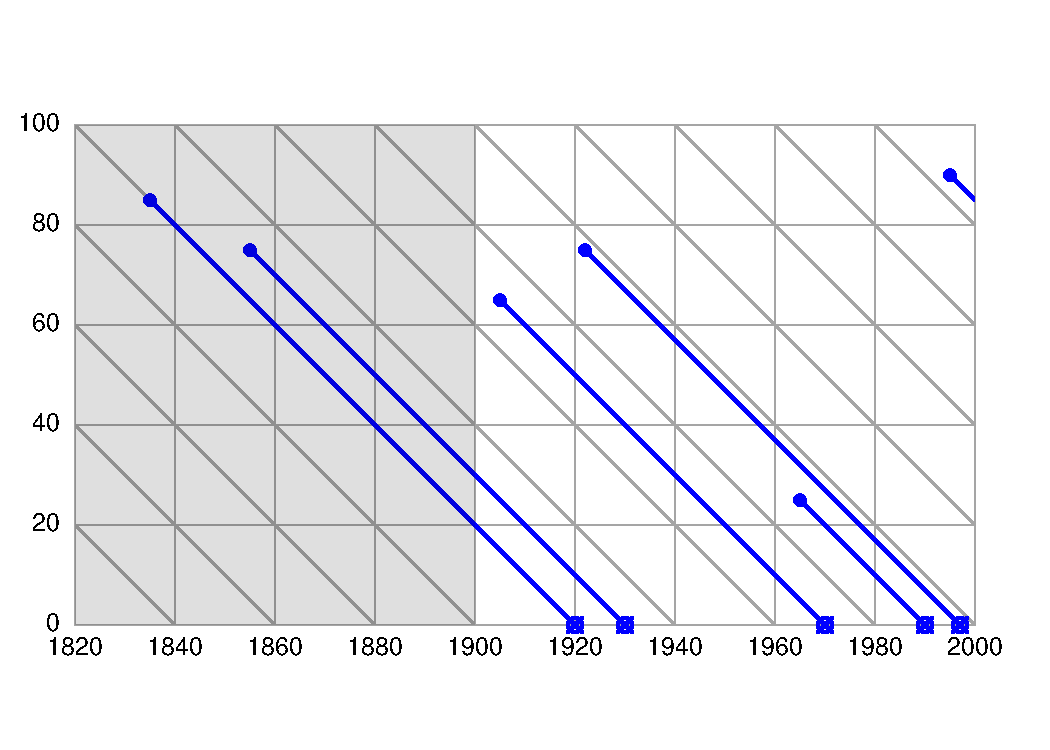
\includegraphics{Figures/LabPres/TPD2.pdf}
    %\caption{Lifelines in the TPD diagram}
\end{figure} 
\end{frame}

% TPD equilateral
\begin{frame}
\frametitle{TPD, equilateral}
\begin{figure}[b]
    \centering
    % figure made in R/TPDlab.R
    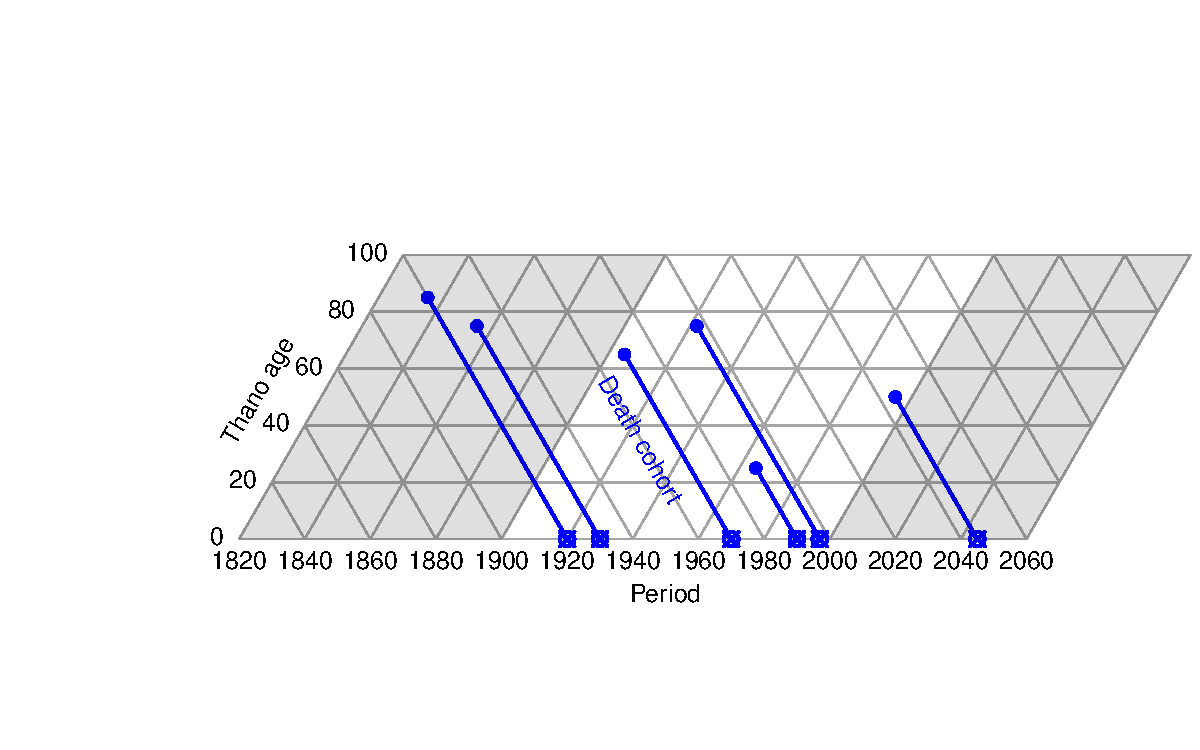
\includegraphics{Figures/LabPres/TPD3.pdf}
\end{figure} 
\end{frame}

\begin{frame}
\frametitle{TPD, \small{spotted in the wild, HT Pancho Villavicencio.}}
\begin{figure}[b]
    \centering
    % figure from elsewhere. Originally produced by myself and Pancho
    % Vilavicencio. This was his most recent version that he used in a
    % presentation at Max-O some weeks ago.
    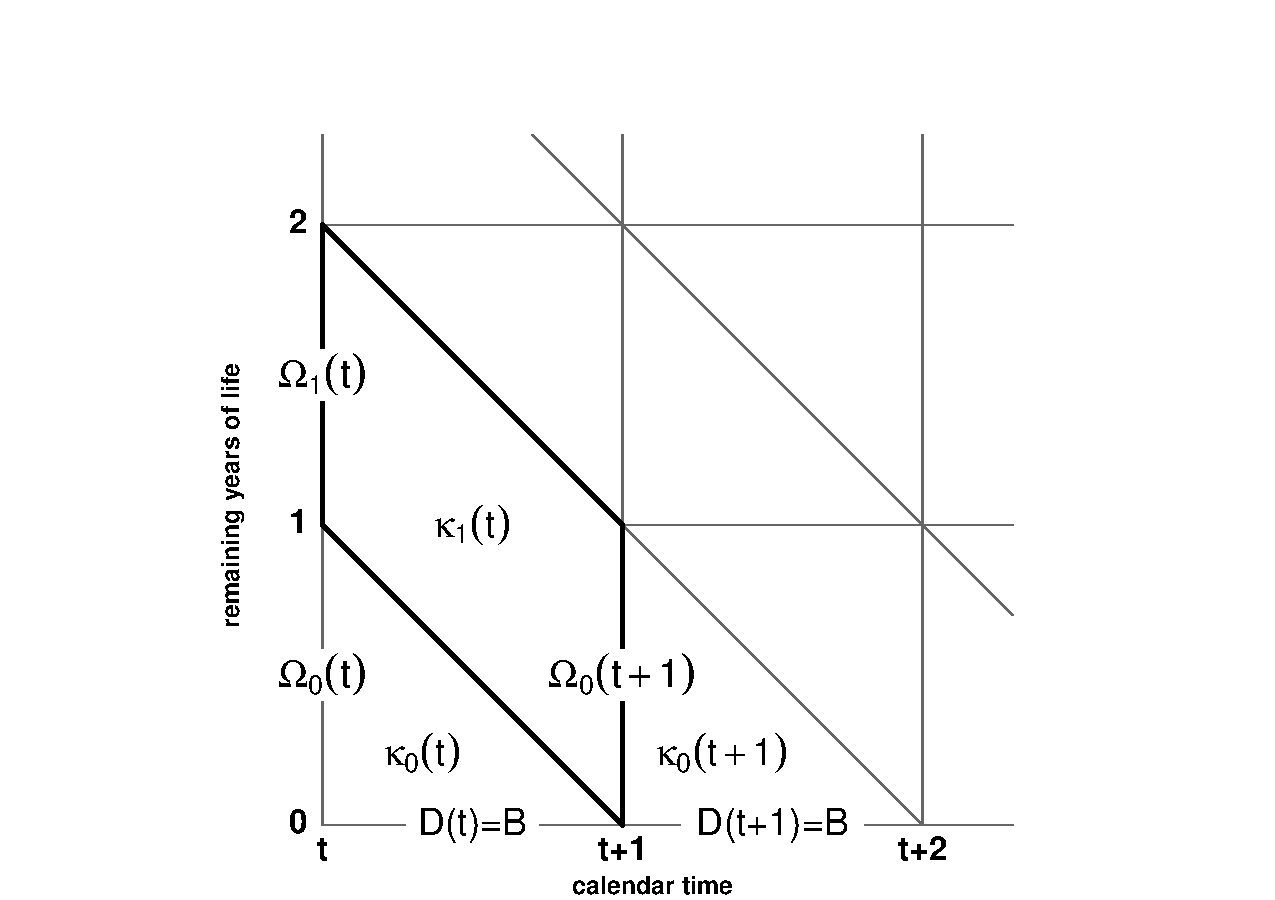
\includegraphics{Figures/LabPres/TPDexample_Pancho.pdf}
\end{figure} 
\end{frame}

%%%%%%%%%%%%%%%%%%%%%%%%%%%%%%%%%%%%%%%%%%%%%%%
\section{ATL}
\begin{frame}
\frametitle{ATL, a lifespan diagram}
\begin{figure}[b]
    \centering
    % figure made in R/ATLlab.R
    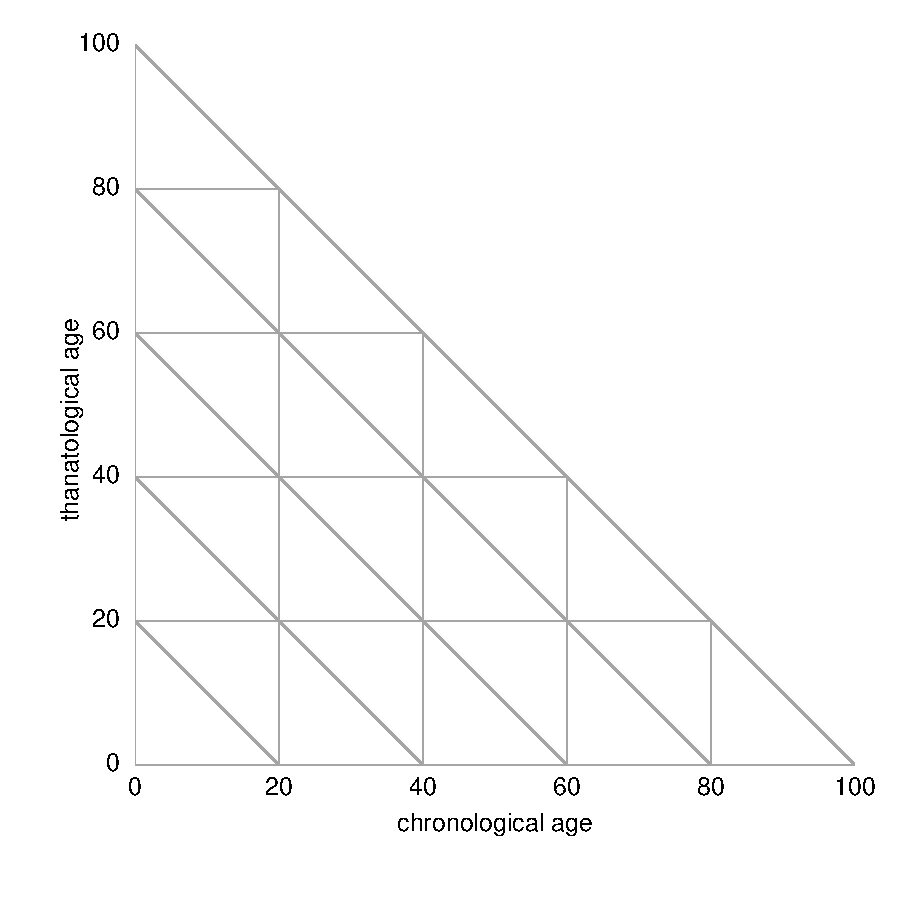
\includegraphics{Figures/LabPres/ATL1.pdf}
\end{figure} 
\end{frame}

% with
\begin{frame}
\frametitle{ATL, a lifespan diagram}
\begin{figure}[b]
    \centering
    % figure made in R/ATLlab.R
    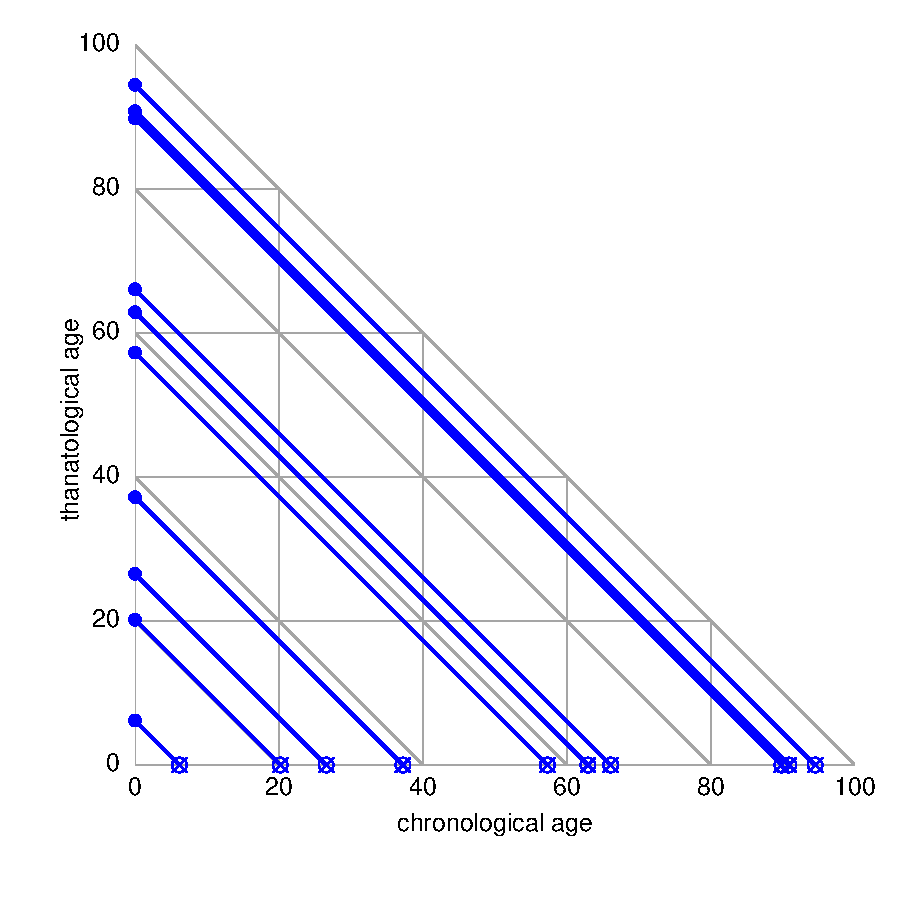
\includegraphics{Figures/LabPres/ATL2.pdf}
\end{figure} 
\end{frame}

\begin{frame}
\frametitle{ATL, a lifespan diagram}
\begin{figure}[b]
    \centering
    % figure made in R/ATLlab.R
    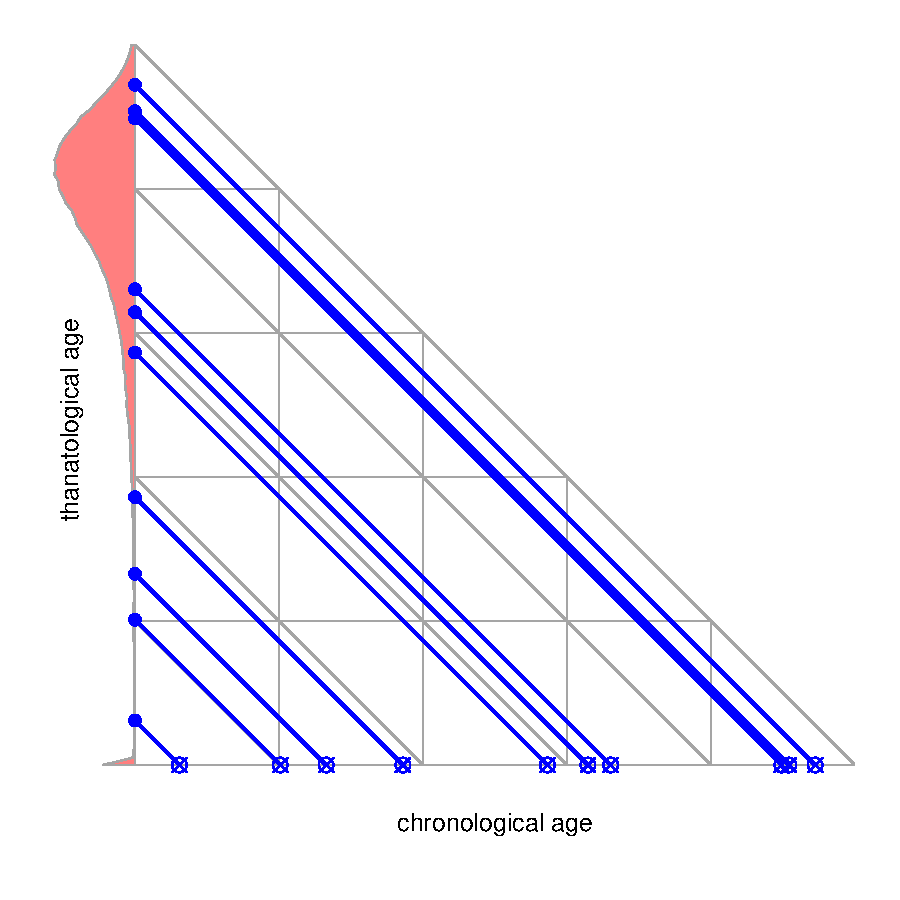
\includegraphics{Figures/LabPres/ATL3.pdf}
\end{figure} 
\end{frame}


\begin{frame}
\frametitle{ATL, a lifespan diagram}
\begin{figure}[b]
    \centering
    % figure made in R/ATLlab.R
    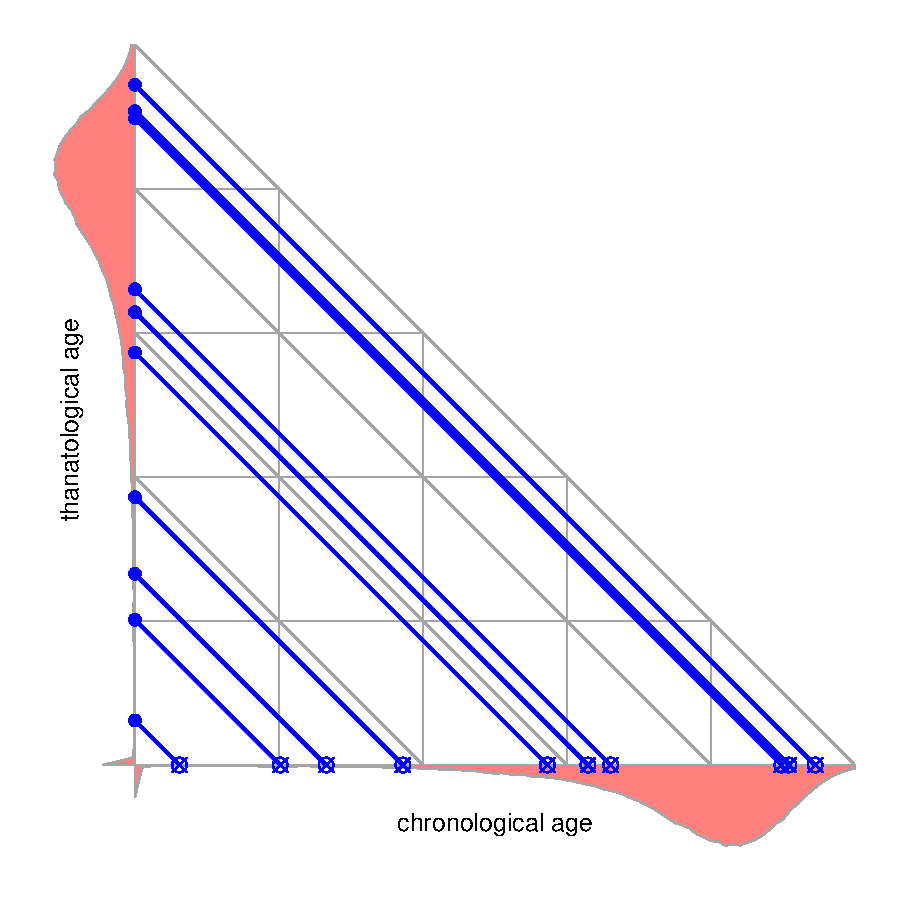
\includegraphics{Figures/LabPres/ATL4.pdf}
\end{figure} 
\end{frame}

\begin{frame}
\frametitle{ATL, a lifespan diagram, cohort}
\begin{figure}[b]
    \centering
    % figure made in R/ATLlab.R
    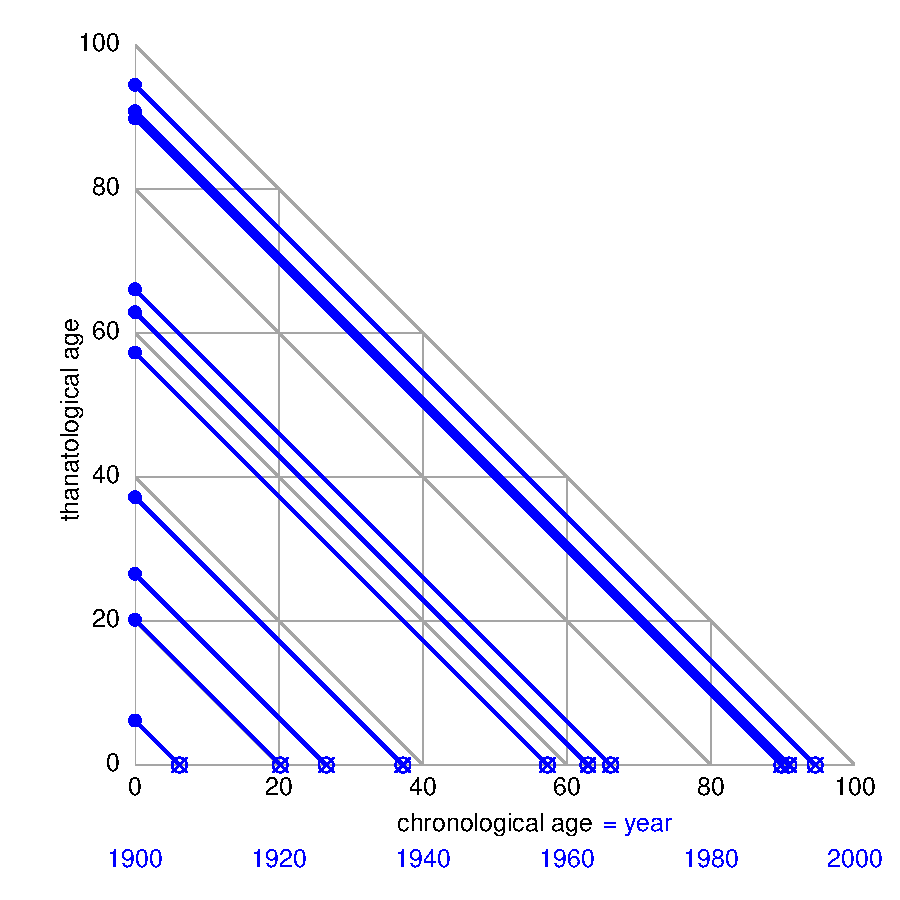
\includegraphics{Figures/LabPres/ATL5.pdf}
    %\caption{Lifelines in the TPD diagram}
\end{figure} 
\end{frame}

\begin{frame}
\frametitle{ATL, a lifespan diagram, cohort, equilateral}
\begin{figure}[b]
    \centering
    % figure made in R/ATLlab.R
    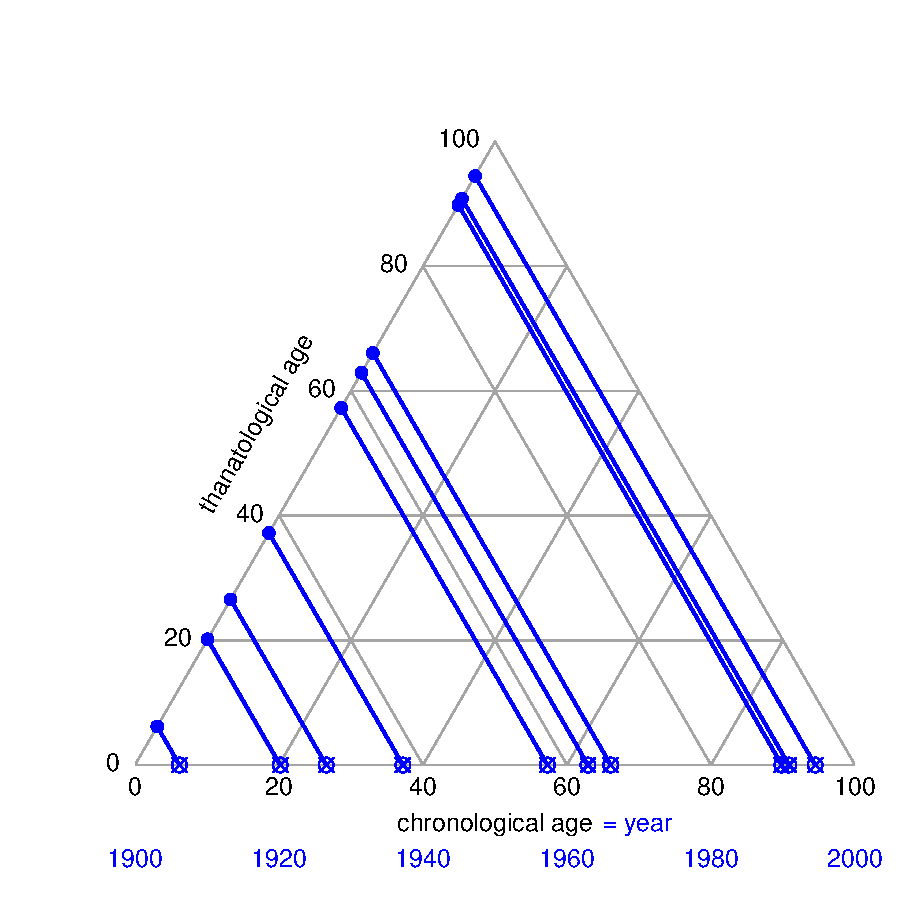
\includegraphics{Figures/LabPres/ATL6.pdf}
\end{figure} 
\end{frame}

\begin{frame}
\frametitle{ATL, cohort, spotted in the wild}
\begin{figure}[b]
    \centering
    % figure made in R/ATLlab.R
    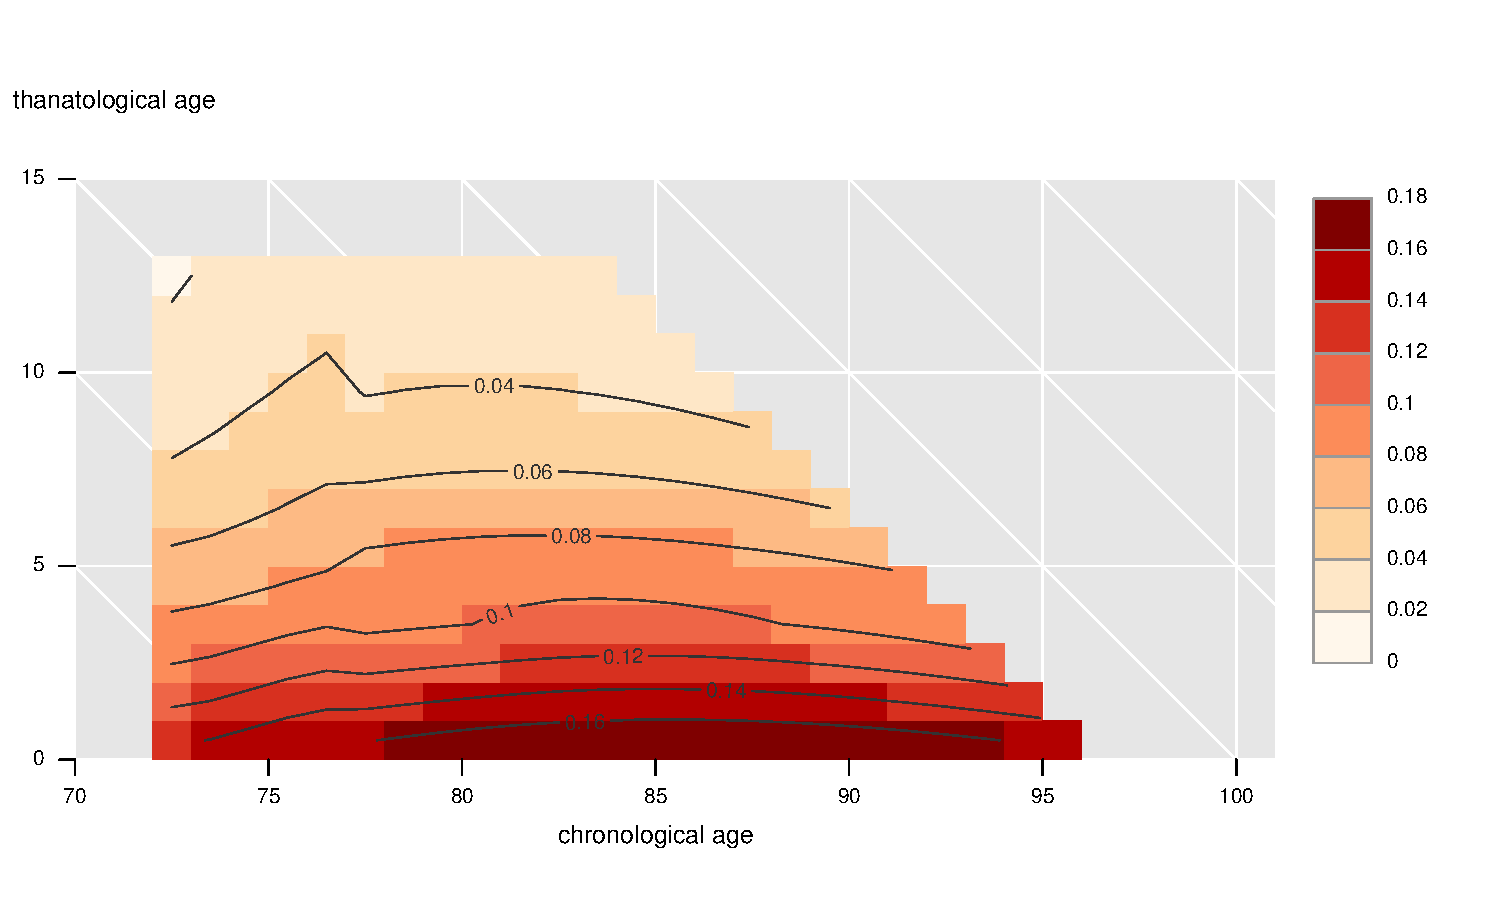
\includegraphics[scale=.9]{Figures/LabPres/ATL_Surf_Male_psych_HRS.pdf}
\end{figure} 
\end{frame}

\section{APCTDL}

\begin{frame}
\frametitle{All diagrams combined:}
Using right-angles (interactive, web):
\url{http://demog.berkeley.edu/~triffe/RGL1/}

\end{frame}

\begin{frame}
\frametitle{All diagrams combined:}

* As a regular honeycomb *

\end{frame}

%%%%%%%%%%%%%%%%%%%%%%%%%%%%%%%%%%%%
\section{Bottled case study}
\begin{frame}[plain]
\begin{figure}[b]
    \raggedright
    % figure made in R/LabChronoDeception.R
    \includegraphics[scale=.7]{Figures/LabPres/CSIRostock.png}
\end{figure}
\end{frame}

\begin{frame}
\frametitle{CSI Rostock}
\begin{figure}[b]
    \centering
    % figure made in R/LabChronoDeception.R
    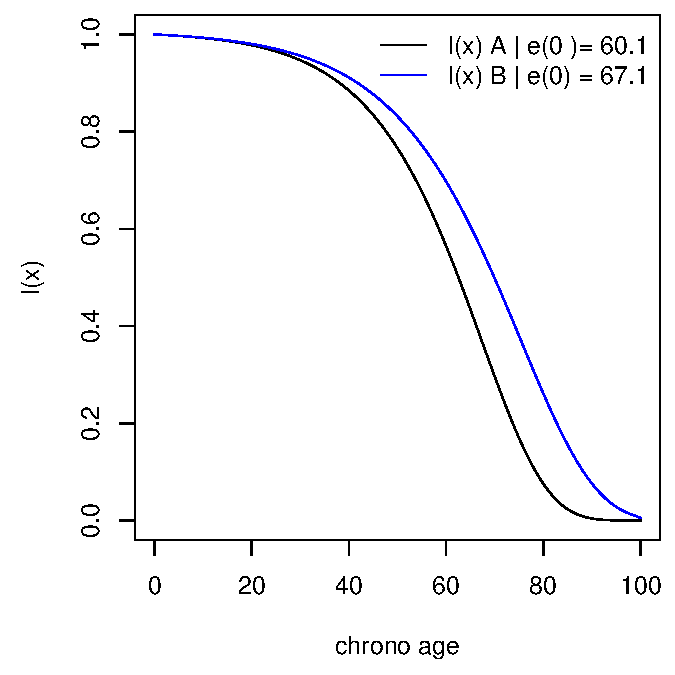
\includegraphics[scale=1.2]{Figures/LabPres/Z1PopAPopB.pdf}
\end{figure} 
\end{frame}

\begin{frame}
\frametitle{CSI Rostock}
\begin{figure}[b]
    \centering
    % figure made in R/LabChronoDeception.R
    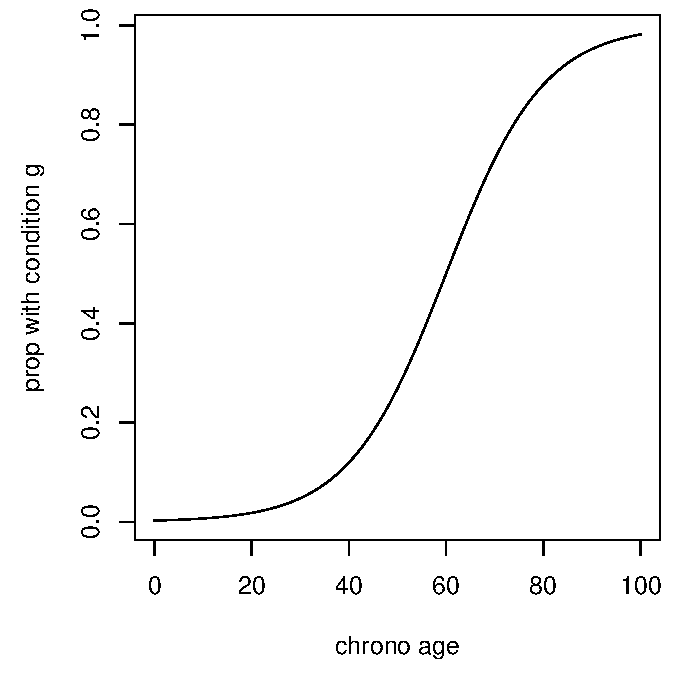
\includegraphics[scale=1.2]{Figures/LabPres/Z2gx.pdf}
\end{figure} 
\end{frame}

\begin{frame}
\frametitle{CSI Rostock}
\begin{figure}[b]
    \centering
    % figure made in R/LabChronoDeception.R
    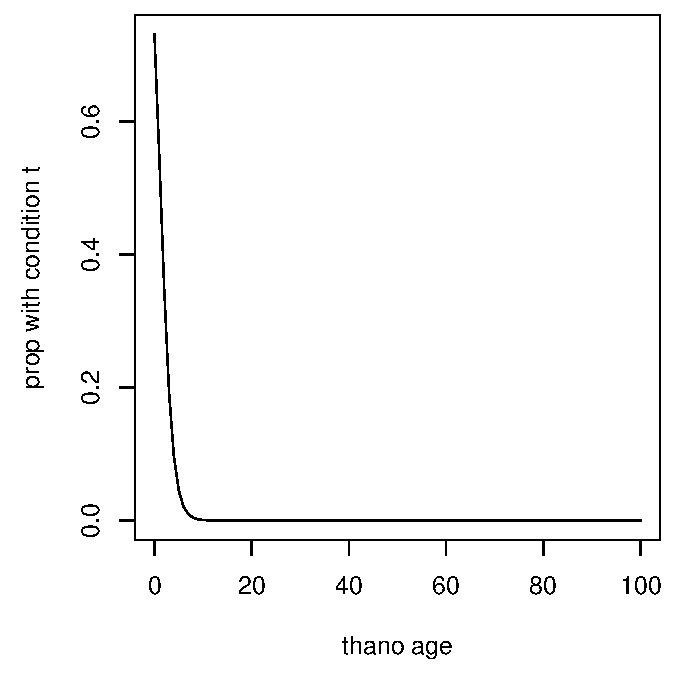
\includegraphics[scale=1.2]{Figures/LabPres/Z3ty.pdf}
\end{figure} 
\end{frame}

\begin{frame}
\frametitle{CSI Rostock}
\begin{figure}[b]
    \centering
    % figure made in R/LabChronoDeception.R
    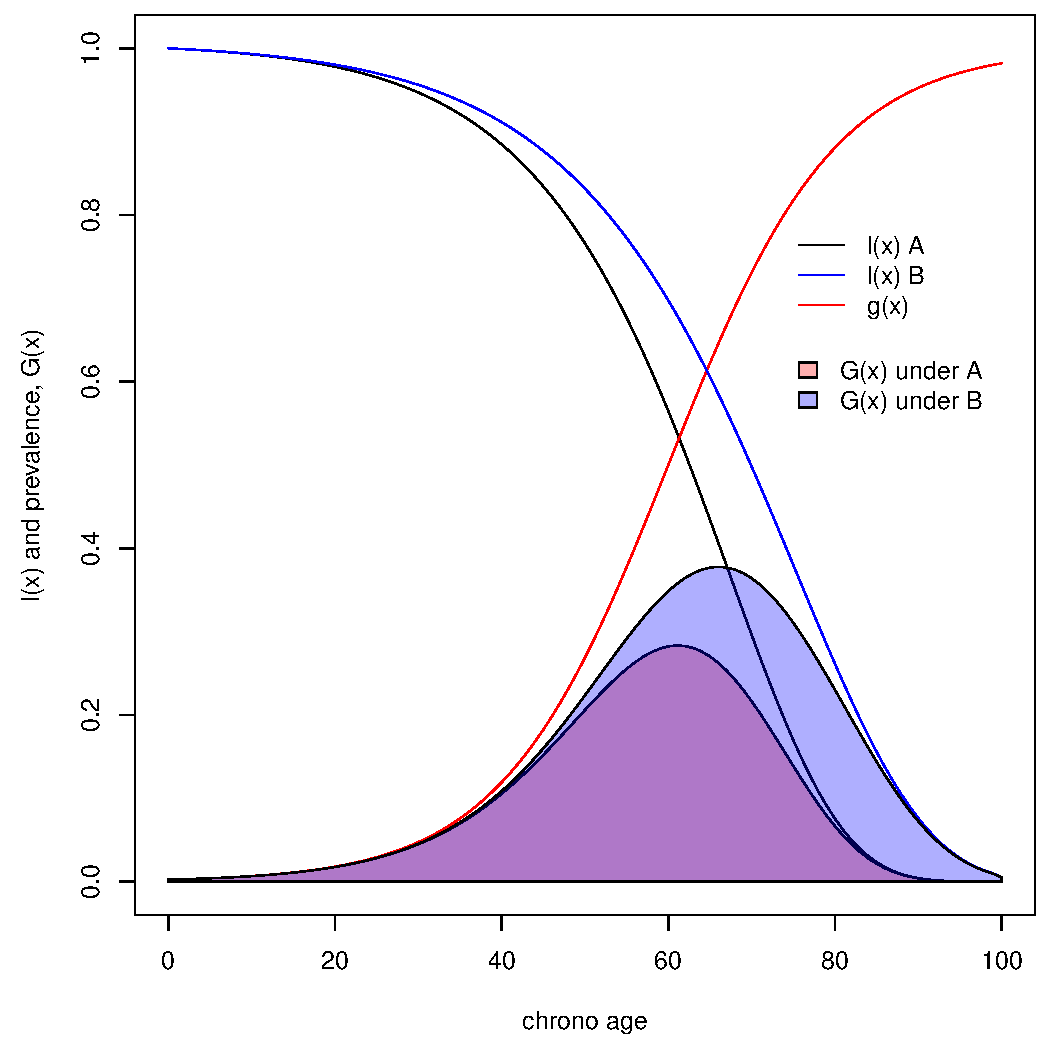
\includegraphics[scale=.9]{Figures/LabPres/Z4GxAB.pdf}
\end{figure} 
\end{frame}

\begin{frame}
\frametitle{CSI Rostock}
\begin{figure}[b]
    \centering
    % figure made in R/LabChronoDeception.R
    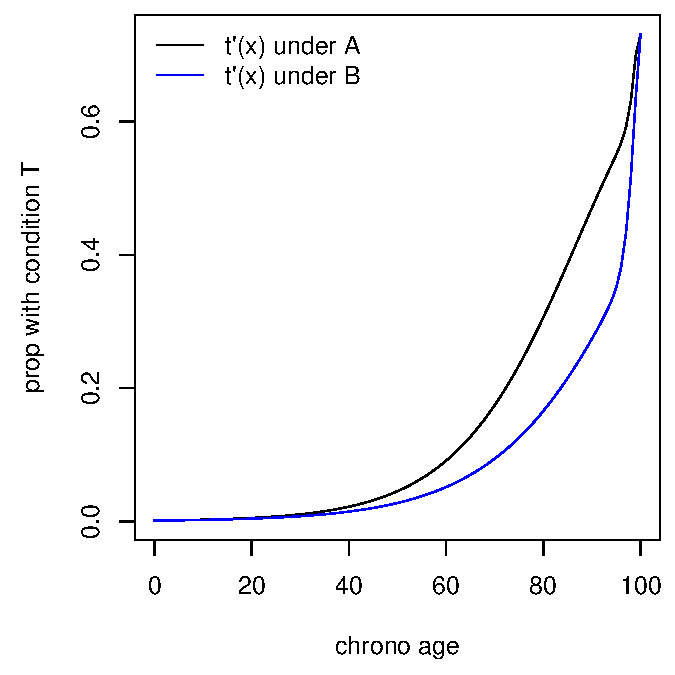
\includegraphics[scale=1.2]{Figures/LabPres/Z5txAtxB.pdf}
\end{figure} 
\end{frame}

\begin{frame}
\frametitle{CSI Rostock}
\begin{figure}[b]
    \centering
    % figure made in R/LabChronoDeception.R
    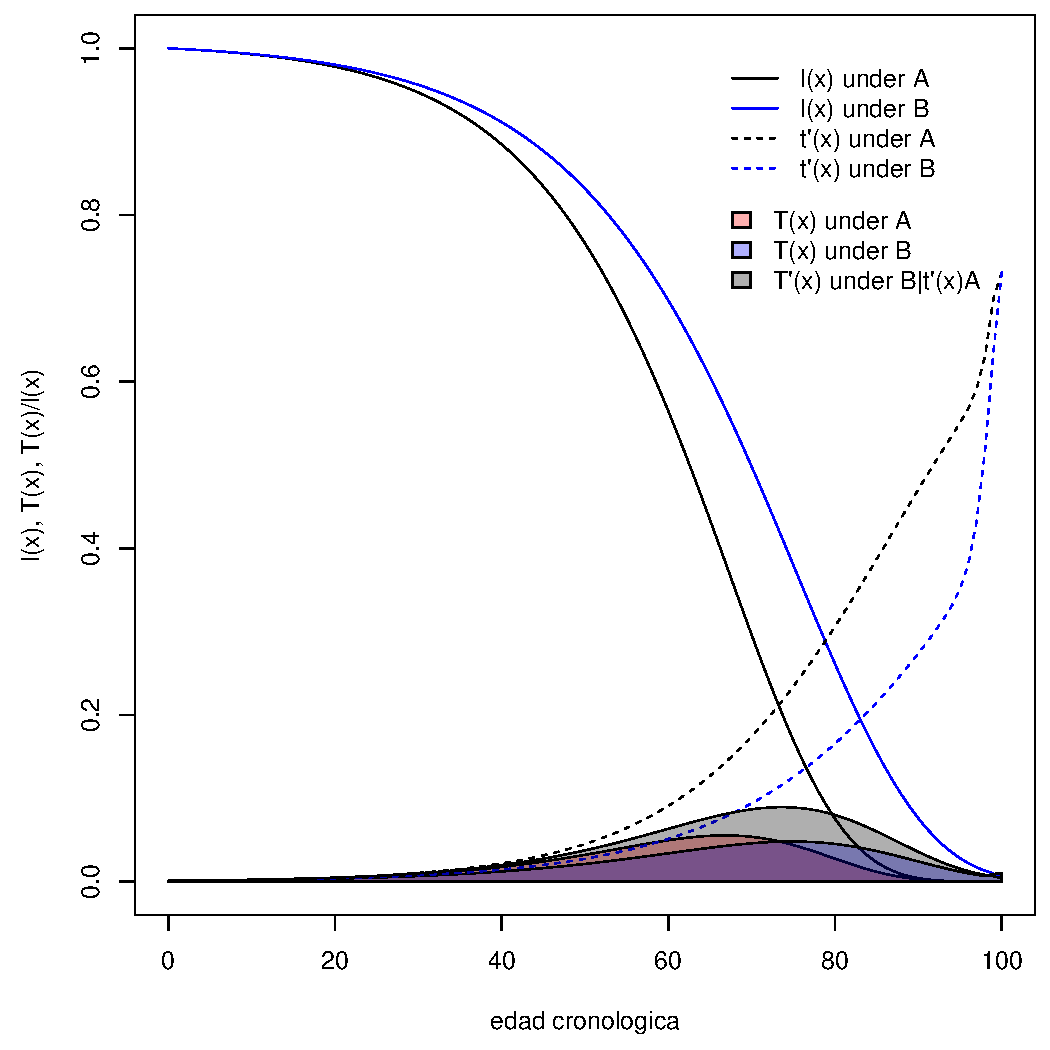
\includegraphics[scale=.9]{Figures/LabPres/Z6TxATxB.pdf}
\end{figure} 
\end{frame}

\begin{frame}
\frametitle{CSI Rostock}
\begin{itemize}
  \item\item<1-> Chrono variation = mortality morbidity tradeoff
  \item\item<2-> Thano variation = win
  \item\item<3-> miscategorizing thano variation leads in wrong direction
  \item\item<4-> assumptions were strong here\ldots
\end{itemize}
\end{frame}
%%%%%%%%%%%%%%%%%%%%%%%%%%%%%%%%%%
%%	End of the document					%%
%%%%%%%%%%%%%%%%%%%%%%%%%%%%%%%%%%
\end{document}










